
\section{Testing}\label{sec:testing}
    \subsection{Testing Plan}
        The primary focus for our testing is to ensure the components we have created work well on a small scale. To accomplish this, we have not yet set up any serious automated testing nor CI/CD integrated with our version control, and instead opted to create small integration tests as needed to speed up prototyping.

        We developed a Go client to confirm the backend worked as expected when experiencing difficulty with gRPC-Web. 

    \subsection{Tests for Functional Requirements}
        We tested creating multiple accounts and edge-cases involving empty input strings and other invalid input. Several edge cases still fail, since we are writing our own validation instead of using an external library.

        Other functional requirements haven't been tested yet because the functionality is not yet there.

    \subsection{Tests for Non-functional Requirements}
        \begin{figure}[h!]
            \centering
            
            \caption{Lighthouse performance audit}
            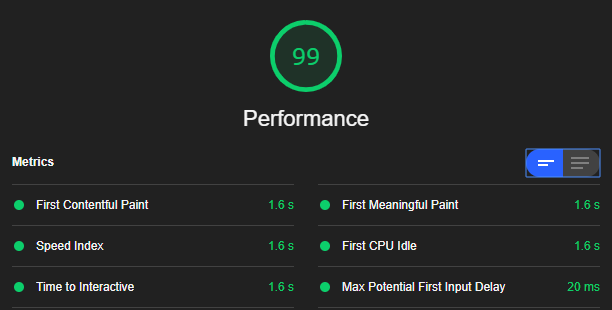
\includegraphics[width=0.7\textwidth]{images/lighthouse.png}
        \end{figure}
    
    \subsection{Hardware and Software Requirements}
        Our Go client runs on the same hardware and software stack as the backend Go server.
